\section{RL for Chip Design}

% Shared colours for this lecture's diagrams
\definecolor{sysblue}{RGB}{189,215,238}
\definecolor{mlgreen}{RGB}{169,208,142}
\definecolor{boxtan}{RGB}{248,203,173}
\definecolor{boxgreen}{RGB}{197,224,180}
\definecolor{boxblue}{RGB}{180,199,231}
\definecolor{boxred}{RGB}{244,177,177}
% prior-approaches method-box colours (match the original slides 10/11)
\definecolor{mpink}{RGB}{244,204,204}
\definecolor{mcream}{RGB}{255,241,204}
\definecolor{mblue}{RGB}{206,225,243}
\definecolor{mgreen}{RGB}{217,234,211}

% ---------------------------------------------------------------- Slide 2
\begin{frame}{RL for Chip Design}
\vfill
\begin{center}
{\footnotesize Article \quad\textbar\quad Published: 09 June 2021}

\vspace{0.6em}
{\LARGE\bfseries \href{https://www.nature.com/articles/s41586-021-03544-w}{A graph placement methodology for fast chip design}}

\vspace{0.8em}
{\footnotesize Azalia Mirhoseini, Anna Goldie, Mustafa Yazgan, Joe Wenjie Jiang,
Ebrahim Songhori, Shen Wang, Young-Joon Lee, Eric Johnson, Omkar Pathak,
Azade Nazi, Jiwoo Pak, Andy Tong, Kavya Srinivasa, William Hang, Emre Tuncer,
Quoc V. Le, James Laudon, Richard Ho, Roger Carpenter \& Jeff Dean}

\vspace{0.8em}
{\footnotesize \textit{Nature} \textbf{594}, 207--212 (2021)}
\end{center}
\vfill
\end{frame}

% ---------------------------------------------------------------- Slide 3
\begin{frame}{In the past decade, systems and hardware have transformed ML.}
\vfill
\begin{center}
\begin{tikzpicture}[font=\large]
    \node[draw, fill=sysblue, minimum width=3.4cm, minimum height=1.5cm] (sys) {Systems};
    \node[draw, fill=mlgreen, minimum width=3.4cm, minimum height=1.5cm, right=3cm of sys] (ml) {ML};
    \draw[-{Stealth[length=3mm]}, gray] (sys.north) to[bend left=45] (ml.north);
\end{tikzpicture}
\end{center}
\vfill
\end{frame}

% ---------------------------------------------------------------- Slide 4
\begin{frame}{\small In the past decade, systems and hardware have transformed ML. Now, it's time for ML to transform systems and hardware.}
\vfill
\begin{center}
\begin{tikzpicture}[font=\large]
    \node[draw, fill=sysblue, minimum width=3.4cm, minimum height=1.5cm] (sys) {Systems};
    \node[draw, fill=mlgreen, minimum width=3.4cm, minimum height=1.5cm, right=3.5cm of sys] (ml) {ML};
    \draw[-{Stealth[length=3mm]}, gray] (sys.north) to[bend left=45] (ml.north);
    \draw[-{Stealth[length=3mm]}, gray] (ml.south) to[bend left=45] (sys.south);
\end{tikzpicture}
\end{center}
\vfill
\end{frame}

% ---------------------------------------------------------------- Slide 5
\begin{frame}{Demand for Compute Outpacing Supply (Moore's Law)}
\begin{columns}[c]
\begin{column}{0.52\textwidth}
\centering
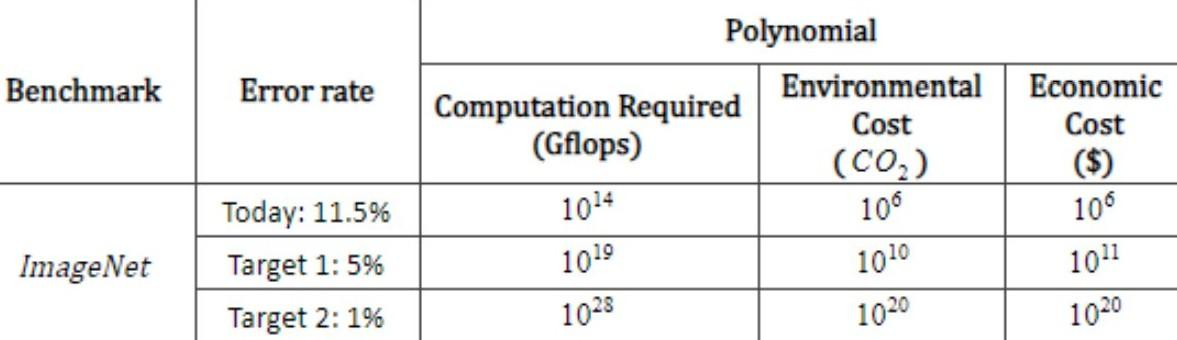
\includegraphics[width=\linewidth,keepaspectratio]{images/rl-real-world/figures/compute-table.jpg}

\vspace{0.4em}
{\tiny Implications of achieving performance on the computation, carbon emissions, and
economic costs from deep learning on projections from polynomial models.
\textit{The Computational Limits of Deep Learning}, Thompson et al., 2020}
\end{column}
\begin{column}{0.48\textwidth}
\centering
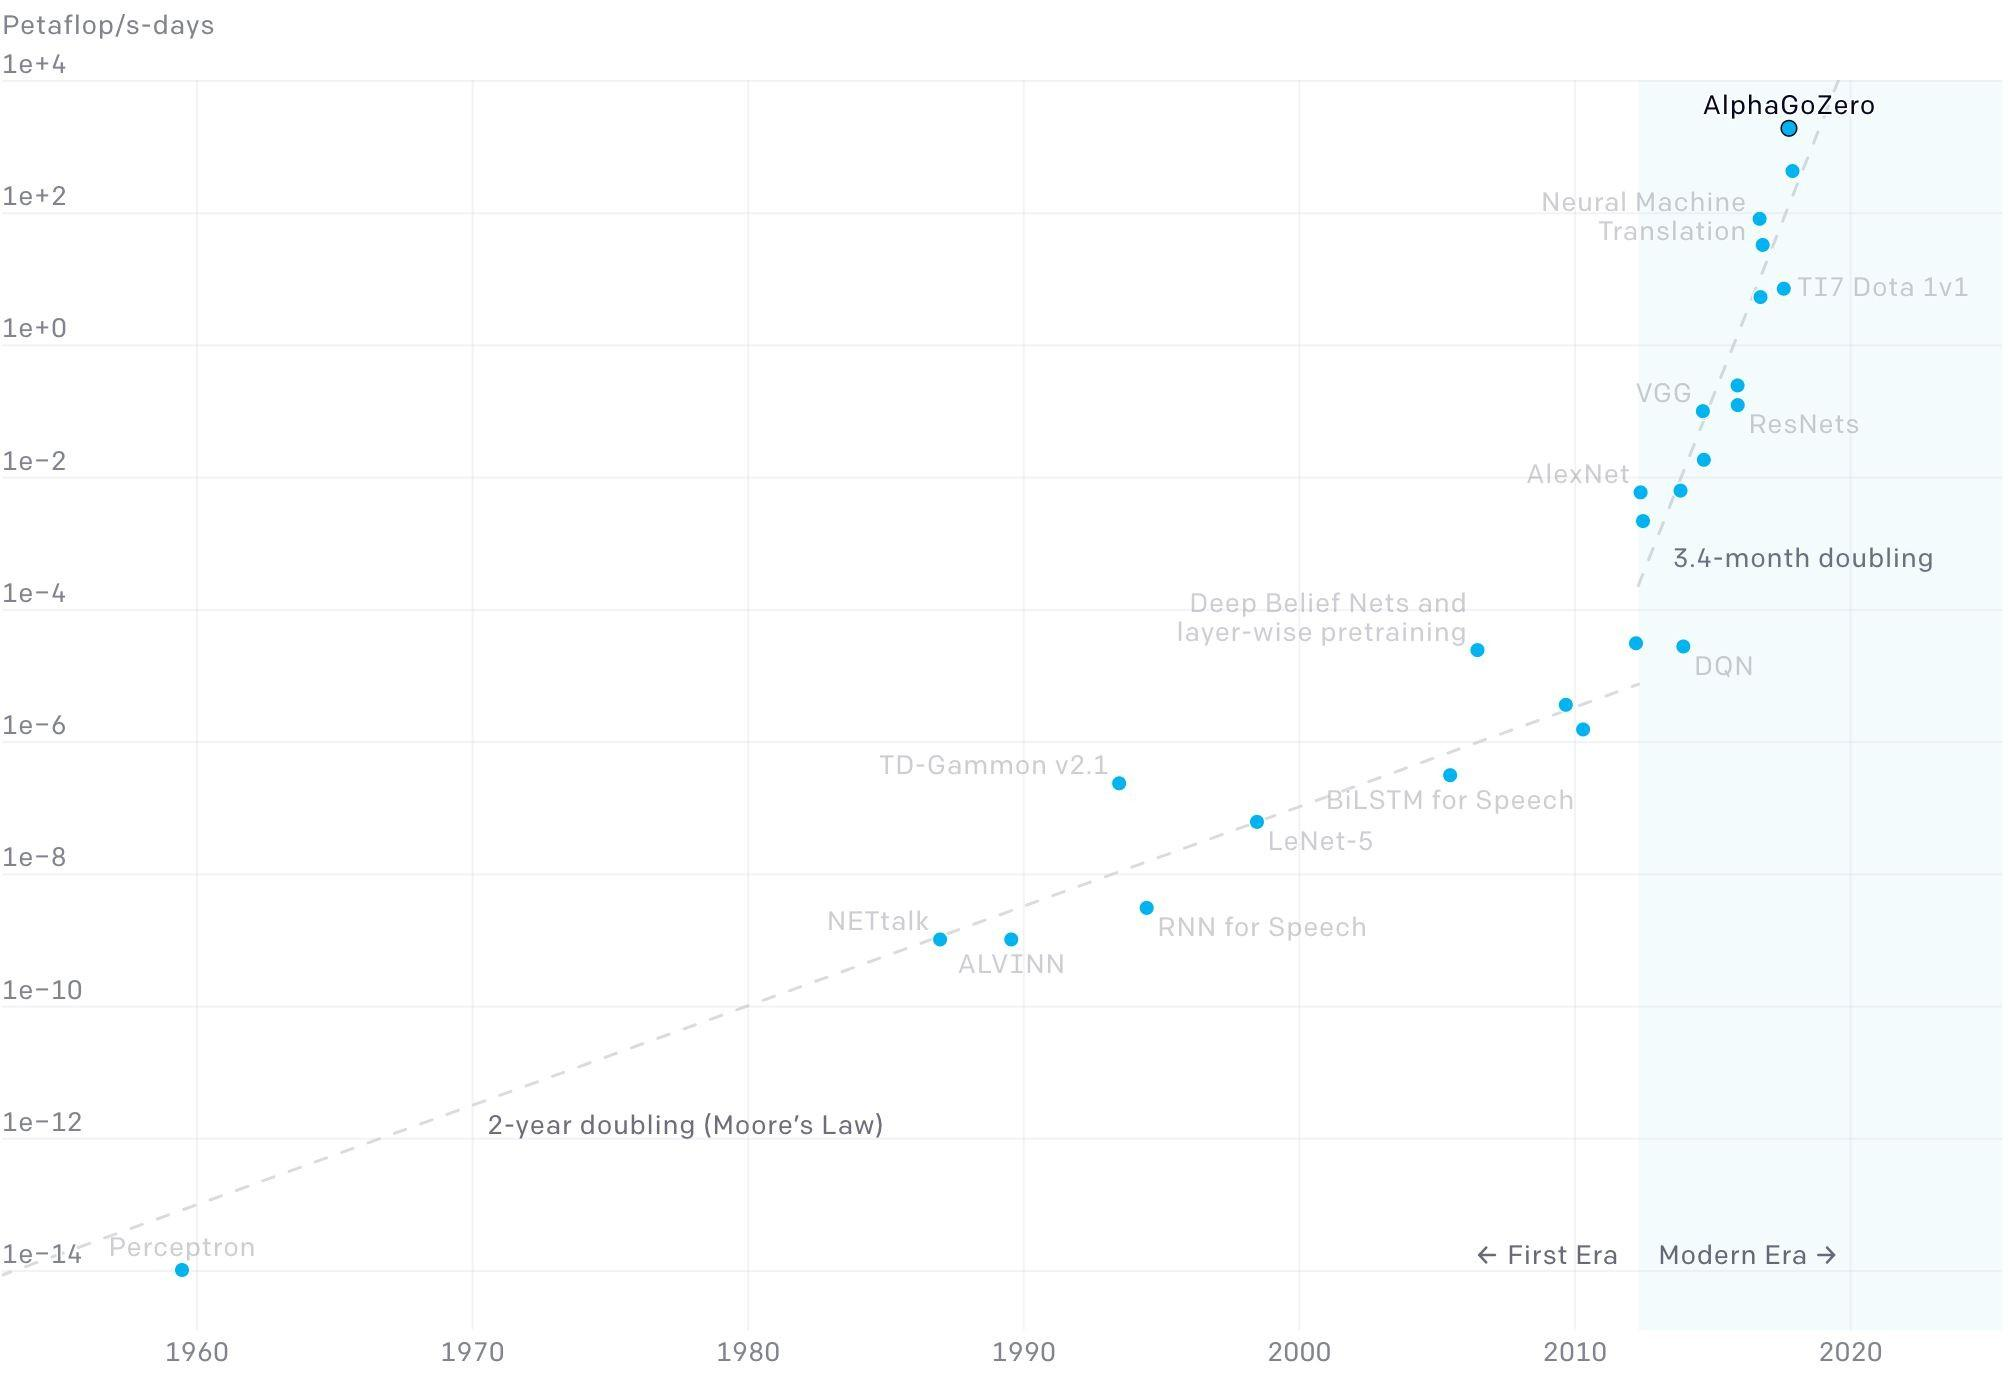
\includegraphics[width=\linewidth,height=0.62\textheight,keepaspectratio]{images/rl-real-world/figures/compute-chart.jpg}

\vspace{0.3em}
{\tiny Since 2012, the amount of compute used in the largest AI training runs doubled
every 3.4 months, OpenAI, 2019}
\end{column}
\end{columns}
\end{frame}

% ---------------------------------------------------------------- Slide 6
\begin{frame}{Scaling Laws: Compute Fuels Progress in ML}
\centering
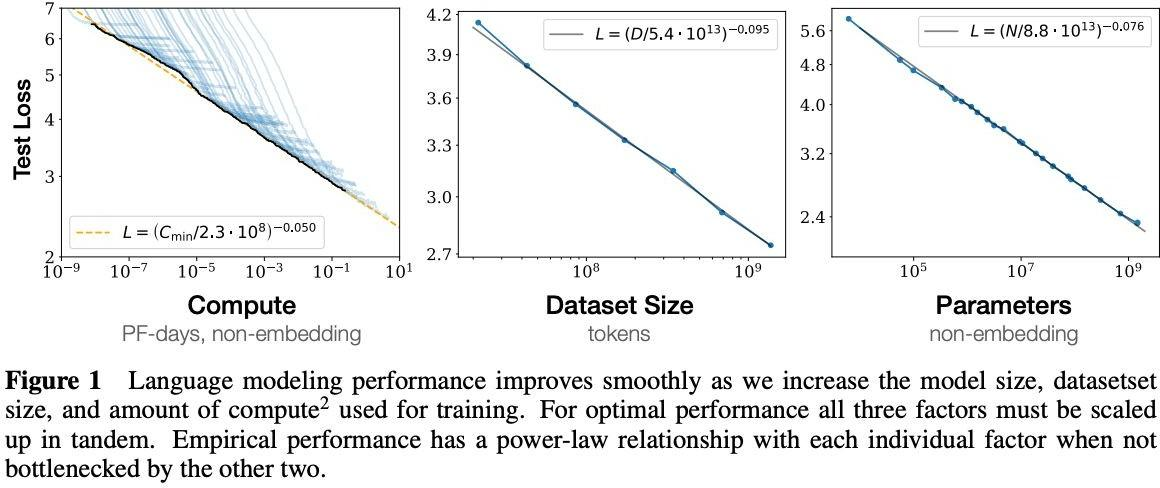
\includegraphics[width=0.96\linewidth,height=0.78\textheight,keepaspectratio]{images/rl-real-world/figures/scaling-laws.jpg}%
\footnote[0]{\scriptsize Kaplan, McCandlish, Henighan, Brown, Chess, Child, Gray, Radford, Wu, Amodei. \href{https://arxiv.org/abs/2001.08361}{Scaling Laws for Neural Language Models}. OpenAI 2020.}
\end{frame}

% ---------------------------------------------------------------- Slide 7
\begin{frame}{Value of Machine Learning for Chip Design}
\begin{itemize}
    \item Enabling cheaper, faster, and more environmentally friendly chips
    \item Potential to reduce the design cycle from 1.5--2 years to weeks
    \begin{itemize}
        \item Today, we design chips for the NN architectures of 2--5 years from now
        \item Shortening the chip design cycle would enable us to be far more adaptive
              to the rapidly advancing field of machine learning
    \end{itemize}
    \item New possibilities emerge if we evolve NN architectures and chips together
    \begin{itemize}
        \item Discovering the next generation of NN architectures (which would not be
              computationally feasible with today's chips)
    \end{itemize}
\end{itemize}
\end{frame}

% ---------------------------------------------------------------- Slide 8
\begin{frame}{Chip Floorplanning Problem}
\begin{itemize}
    \item A form of graph resource optimization
    \item Place the chip components to minimize the latency of computation, power
          consumption, chip area and cost, while adhering to constraints, such as
          congestion, cell utilization, heat profile, etc.
\end{itemize}
\vfill
\centering
\definecolor{pinblue}{RGB}{40,60,200}
\resizebox{\linewidth}{!}{%
\begin{tikzpicture}[
    pin/.style={draw, fill=pinblue, minimum width=0.34cm, minimum height=0.20cm, inner sep=0},
    port/.style={draw, fill=red, minimum width=0.36cm, minimum height=0.24cm, inner sep=0},
    wire/.style={line width=1.2pt, line cap=round},
    lbl/.style={font=\small}]

    % chip canvas
    \fill[black!6] (0.7,0.2) rectangle (15.0,4.6);
    \draw[line width=1pt] (0.7,0.2) rectangle (15.0,4.6);

    % macros (green)
    \node[draw, fill=mlgreen, minimum width=3.6cm, minimum height=2.6cm] (m0) at (4.8,1.9) {};
    \node[draw, fill=mlgreen, minimum width=3.7cm, minimum height=2.6cm] (m1) at (11.35,2.4) {};
    % stand-cells (blue)
    \node[draw, fill=sysblue, minimum width=1.9cm, minimum height=0.6cm] (s0) at (4.3,4.0) {};
    \node[draw, fill=sysblue, minimum width=1.9cm, minimum height=0.6cm] (s1) at (8.3,4.0) {};

    % pins
    \node[pin] (p0m0) at (3.0,2.1) {};
    \node[pin] (p1m0) at (6.6,2.3) {};
    \node[pin] (p0m1) at (9.5,2.3) {};
    \node[pin] (p1m1) at (13.2,2.3) {};
    % ports
    \node[port] (port0) at (0.25,2.1) {};
    \node[port] (port1) at (15.25,4.3) {};

    % ===== nets =====
    % Port P0 -> Stdcell(S0) and P0_M0
    \draw[wire] (port0.east) -- (2.0,2.1);
    \draw[wire] (2.0,2.1) -- (2.0,4.0) -- (s0.west);
    \draw[wire] (2.0,2.1) -- (p0m0.west);
    % Stdcell(S0) -> Stdcell(S1)
    \draw[wire] (s0.east) -- (s1.west);
    % Stdcell(S1) -> P1_M0 -> P0_M1
    \draw[wire] (s1.south) -- (8.3,2.3);
    \draw[wire] (8.3,2.3) -- (p1m0.east);
    \draw[wire] (8.3,2.3) -- (p0m1.west);
    % P1_M1 -> Port P1
    \draw[wire] (p1m1.east) -- (14.6,2.3) -- (14.6,4.3) -- (port1.west);

    % ===== labels =====
    \node[lbl] at (4.45,2.75) {Macro(M0)};
    \node[lbl] at (11.35,3.25) {Macro(M1)};
    \node[lbl] at (4.3,4.0) {Stdcell(S0)};
    \node[lbl] at (8.3,4.0) {Stdcell(S1)};
    \node[lbl] at (3.55,1.8) {P0\_M0};
    \node[lbl] at (5.85,2.6) {P1\_M0};
    \node[lbl] at (10.25,1.95) {P0\_M1};
    \node[lbl] at (12.55,1.95) {P1\_M1};
    \node[lbl, anchor=east] at (0.6,2.62) {Port P0};
    \node[lbl] at (15.0,4.95) {Port P1};
    % macro-pin annotation
    \node[lbl] (mpin) at (7.5,3.05) {Macro pin};
    \draw[-{Stealth[length=2.5mm]}, line width=0.8pt] (7.15,2.9) -- (6.66,2.45);
\end{tikzpicture}%
}
\end{frame}

% ---------------------------------------------------------------- Slide 9
\begin{frame}{Complexity of Chip Placement Problem}
\vfill
\begin{columns}[t]
\begin{column}{0.32\textwidth}
\centering
{\large Chess}\\[0.4em]
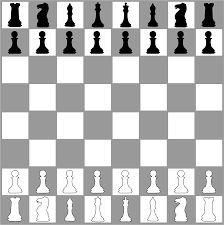
\includegraphics[width=0.7\linewidth]{images/rl-real-world/figures/chess.jpg}\\[0.6em]
Number of states $\sim$\\ $10^{123}$
\end{column}
\begin{column}{0.32\textwidth}
\centering
{\large Go}\\[0.4em]
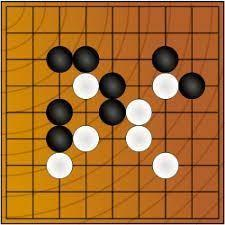
\includegraphics[width=0.7\linewidth]{images/rl-real-world/figures/go.jpg}\\[0.6em]
Number of states $\sim$\\ $10^{360}$
\end{column}
\begin{column}{0.32\textwidth}
\centering
{\large Chip Placement}\\[0.4em]
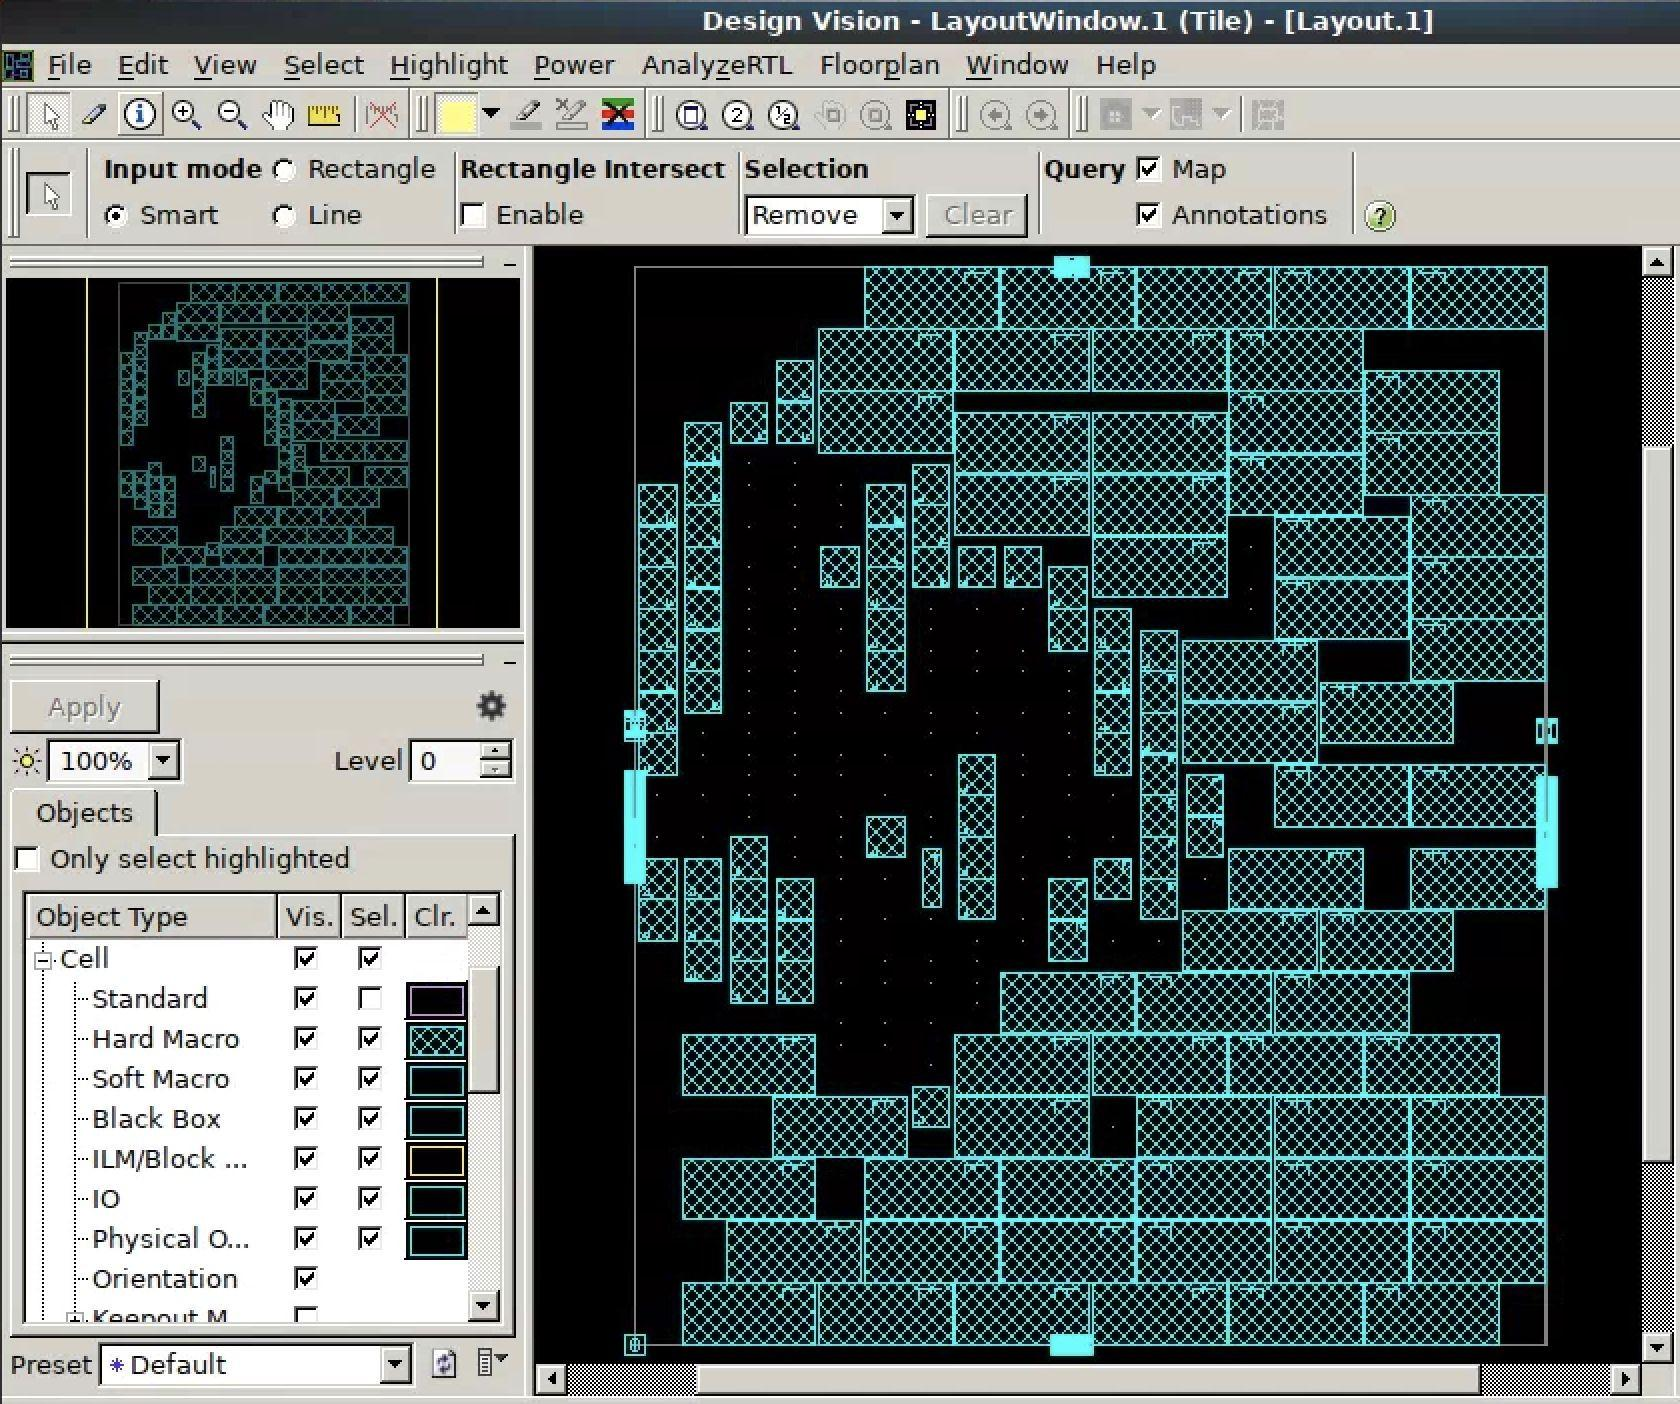
\includegraphics[width=0.95\linewidth]{images/rl-real-world/figures/chip-states.jpg}\\[0.6em]
Number of states $\sim$\\ $10^{9000}$
\end{column}
\end{columns}
\vfill
\end{frame}

% ---------------------------------------------------------------- Slide 10
\begin{frame}{Prior Approaches to Chip Placement}
\vfill
\begin{center}
\begin{tikzpicture}[font=\small,
    pbox/.style={draw, rounded corners, text width=4.6cm, align=center, minimum height=1.6cm}]
    \node[pbox, fill=mpink]   (part) {Partitioning-Based Methods\\(e.g.\ MinCut)};
    \node[pbox, fill=mcream, right=1.2cm of part] (stoch) {Stochastic/Hill-Climbing Methods\\(e.g.\ Simulated Annealing)};
    \node[pbox, fill=mblue, below=1cm of part] (ana) {Analytic Solvers\\(e.g.\ RePlAce)};
\end{tikzpicture}
\end{center}
\vfill
\end{frame}

% ---------------------------------------------------------------- Slide 11
\begin{frame}{Prior Approaches to Chip Placement}
\vfill
\begin{center}
\begin{tikzpicture}[font=\small,
    pbox/.style={draw, rounded corners, text width=4.6cm, align=center, minimum height=1.6cm}]
    \node[pbox, fill=mpink]   (part) {Partitioning-Based Methods\\(e.g.\ MinCut)};
    \node[pbox, fill=mcream, right=1.2cm of part] (stoch) {Stochastic/Hill-Climbing Methods\\(e.g.\ Simulated Annealing)};
    \node[pbox, fill=mblue, below=1cm of part] (ana) {Analytic Solvers\\(e.g.\ RePlAce)};
    \node[pbox, fill=mgreen, below=1cm of stoch] (learn) {Learning-Based Methods};
\end{tikzpicture}
\end{center}
\vfill
\end{frame}

% ---------------------------------------------------------------- Slide 12
\begin{frame}{Chip Placement with Reinforcement Learning}
\begin{columns}[c]
\begin{column}{0.42\textwidth}
\textbf{State:} Graph embedding of chip netlist, embedding of the current node,
and the canvas.
\vspace{1em}

\textbf{Action:} Placing the current node onto a grid cell.
\vspace{1em}

\textbf{Reward:} A weighted average of total wirelength, density, and congestion.
\end{column}
\begin{column}{0.58\textwidth}
\centering
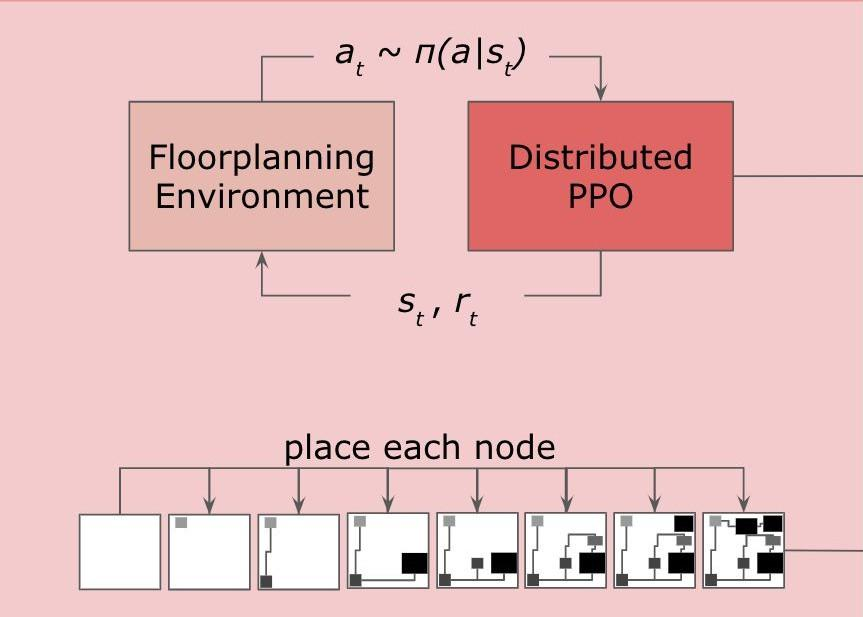
\includegraphics[width=\linewidth,height=0.74\textheight,keepaspectratio]{images/rl-real-world/figures/chip-rl-diagram.jpg}
\end{column}
\end{columns}
\end{frame}

% ---------------------------------------------------------------- Slide 13
\begin{frame}{The Objective Function}
\vfill
\begin{equation*}
    J(\theta, G) \;=\; \frac{1}{K} \sum_{g \sim G}
        \mathbb{E}_{p \sim \pi_\theta}\!\left[ R_{p,g} \right]
\end{equation*}
\vspace{0.5em}
\begin{itemize}\footnotesize
    \item $G$: set of training graphs, $\;K$: size of the training set
    \item $\pi_\theta$: RL policy parameterized by $\theta$
    \item $R_{p,g}$: reward corresponding to placement $p$ of netlist (graph) $g$
\end{itemize}
\vfill
\begin{equation*}
    R_{p,g} \;=\; -\,\text{Wirelength}(p,g)
        \;-\; \lambda\,\text{Congestion}(p,g)
        \;-\; \gamma\,\text{Density}(p,g)
\end{equation*}
\vfill
\end{frame}

% ---------------------------------------------------------------- Slide 14
\begin{frame}{A Hybrid Approach to Placement Optimization}
\vfill
\centering
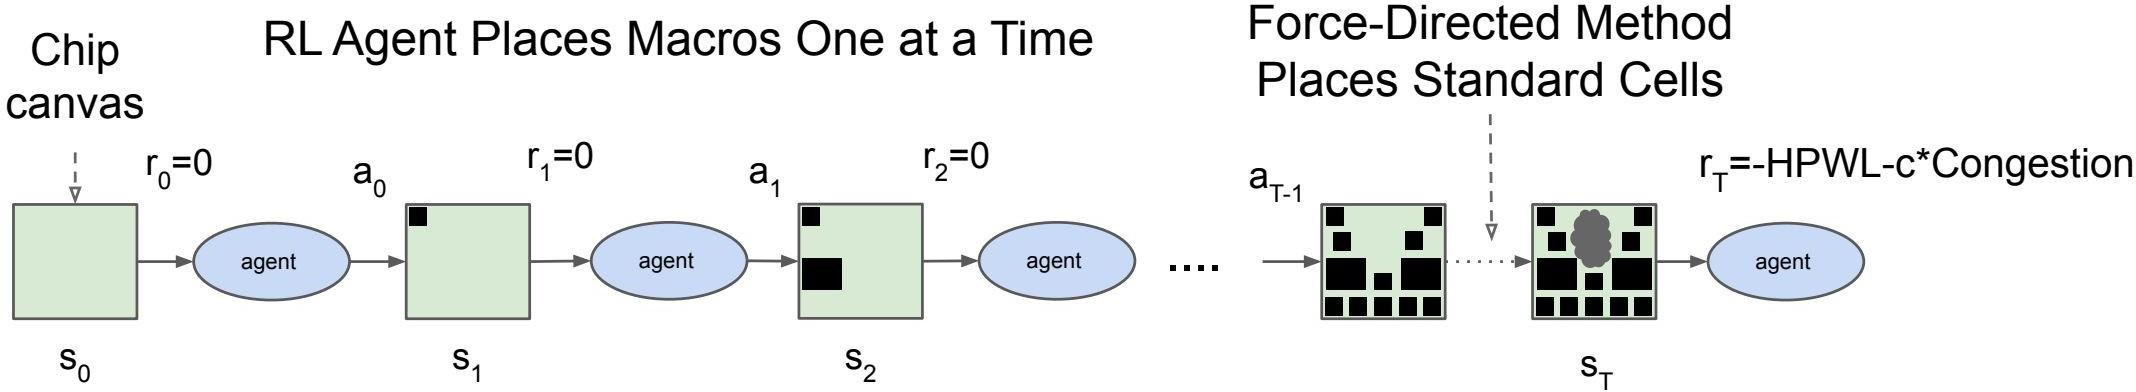
\includegraphics[width=\linewidth,keepaspectratio]{images/rl-real-world/figures/hybrid-approach.jpg}
\vfill
\end{frame}

% ---------------------------------------------------------------- Slide 15
\begin{frame}{Results on a TPU-v4 Block}
\centering
{\footnotesize White area are macros and the green area is composed of standard cell
clusters. The agent finds smoother, rounder macro placements to reduce the wirelength.}
\vfill
\begin{columns}[t]
\begin{column}{0.5\textwidth}
\centering
\textbf{Human Expert}\\[0.3em]

\includegraphics[width=0.78\linewidth]{images/rl-real-world/figures/tpu-human.jpg}\\[0.4em]
{\scriptsize
Time taken: $\sim$6--8 weeks\\
Total wirelength: 57.07m\\
Route DRC* violations: 1766}
\end{column}
\begin{column}{0.5\textwidth}
\centering
\textbf{ML Placer}\\[0.3em]

\includegraphics[width=0.78\linewidth]{images/rl-real-world/figures/tpu-ml.jpg}\\[0.4em]
{\scriptsize
Time taken: 24 hours\\
Total wirelength: 55.42m ($-2.9\%$ shorter)\\
Route DRC violations: 1789 ($+23$ -- negligible difference)}
\end{column}
\end{columns}
\vfill
{\tiny *DRC: Design Rule Checking}
\end{frame}

% ---------------------------------------------------------------- Slide 16
\begin{frame}{Moving Towards Generalized Placements}
\centering
\resizebox{0.92\linewidth}{!}{%
\begin{tikzpicture}[font=\scriptsize,
    hdr/.style={align=center, text width=5.6cm, font=\footnotesize},
    gb/.style={draw, rounded corners, fill=boxgreen, minimum width=1.7cm, minimum height=1.0cm, align=center},
    rb/.style={draw, rounded corners, fill=boxred,   minimum width=1.7cm, minimum height=1.0cm, align=center},
    txt/.style={align=center},
    ar/.style={-{Stealth[length=2mm]}, thick},
    loop/.style={-{Stealth[length=2mm]}}]

% ===================== headers =====================
\node[hdr] at (2.85,6.5) {\textbf{Before:} Training from scratch for each chip netlist};
\node[hdr] at (9.8,6.5)  {\textbf{Then:} Pre-training the policy and fine-tuning on new netlists};

% ===================== BEFORE panel =====================
\draw[gray] (-0.3,-0.4) rectangle (6.0,5.4);
\node[txt] at (2.85,5.0) {Training \hspace{1.2cm} Training};
\node[txt] (nl)  at (0.5,2.7) {New\\Netlist};
\node[gb]  (pol) at (2.3,2.7) {Placer\\Policy};
\node[rb]  (pl)  at (4.3,2.7) {Placements};
\node[txt] (res) at (5.6,3.4) {Final\\result};
\draw[ar] (nl)  -- (pol);
\draw[ar] (pol) -- (pl);
\draw[ar] (pl.east) -- (res);
% feedback loop drawn below
\draw[loop] (pl.south) -- ++(0,-0.7) -| (pol.south);
\node[txt, font=\tiny] at (3.3,1.55) {10,000s of iterations};

% ===================== THEN: training sub-panel =====================
\draw[gray] (6.6,2.6) rectangle (13.0,5.4);
\node[txt] (k1) at (7.4,4.8) {Netlist 1};
\node[txt] (k2) at (7.4,4.1) {Netlist 2};
\node[txt] (kn) at (7.4,3.3) {Netlist N};
\node[gb] (tpol) at (9.5,4.05) {Policy};
\node[rb] (tpl)  at (11.6,4.05) {Placements};
\draw[ar] (k1.east) -- (tpol);
\draw[ar] (k2.east) -- (tpol);
\draw[ar] (kn.east) -- (tpol);
\draw[ar] (tpol) -- (tpl);
\draw[loop] (tpl.south) -- ++(0,-0.5) -| (tpol.south);
\node[txt, font=\tiny] at (10.5,3.15) {10,000s of iterations};

% ===================== THEN: inference sub-panel =====================
\draw[gray] (6.6,-0.4) rectangle (13.0,2.4);
\node[txt] at (9.8,2.0) {Inference};
\node[txt] (inl)  at (7.5,0.9) {New\\Netlist};
\node[gb]  (ipol) at (9.5,0.9) {Pre-Trained\\Policy};
\node[rb]  (ipl)  at (11.6,0.9) {Placements};
\node[txt] (ires) at (12.7,1.55) {Final\\result};
\draw[ar] (inl)  -- (ipol);
\draw[ar] (ipol) -- (ipl);
\draw[ar] (ipl.east) -- (ires);
\draw[loop] (ipl.south) -- ++(0,-0.45) -| (ipol.south);
\node[txt, font=\tiny] at (10.5,0.05) {100s of iterations};
\end{tikzpicture}%
}
\end{frame}

% ---------------------------------------------------------------- Slide 17
\begin{frame}{Achieved generalization by Training Accurate Reward Predictors}
\textbf{Key observation:} A value network trained only on placements generated by a
single policy is unable to accurately predict the quality of placements generated by
another policy, limiting the ability of the policy network to generalize.
\vfill
To decompose the problem, they trained models capable of accurately predicting reward
from off-policy data. \textit{(Inverse RL)}
\end{frame}
